\setstretch{1}
\setlength{\parskip}{\baselineskip}

\setcounter{chapter}{7} % Sets the internal count to 4
\chapter{Benchmarking and Validation} % This will compile as Chapter 5

% --- Settings for SPICE Netlists ---
\lstset{
    basicstyle=\ttfamily\small,
    breaklines=true,
    frame=single,
    backgroundcolor=\color{gray!5},
    keywordstyle=\color{blue},
    commentstyle=\color{gray},
    captionpos=b,
    showstringspaces=false
}

% ==========================================
% SECTION 1: FULL-WAVE BRIDGE RECTIFIER
% ==========================================
\section{Full-Wave Bridge Rectifier}

\subsection{Objective}
The purpose of this test is to validate the correctness of the transient analysis engine, diode device model implementation, waveform generation, and post-processing measurement utilities. The results produced by the developed simulator are compared with those from ngspice.

\subsection{Circuit Description}
The test circuit is a full-wave bridge rectifier consisting of:
\begin{itemize}
    \item AC sinusoidal voltage source
    \item Four-diode bridge rectifier
    \item Load resistor
\end{itemize}

\begin{figure}[H]
    \centering
    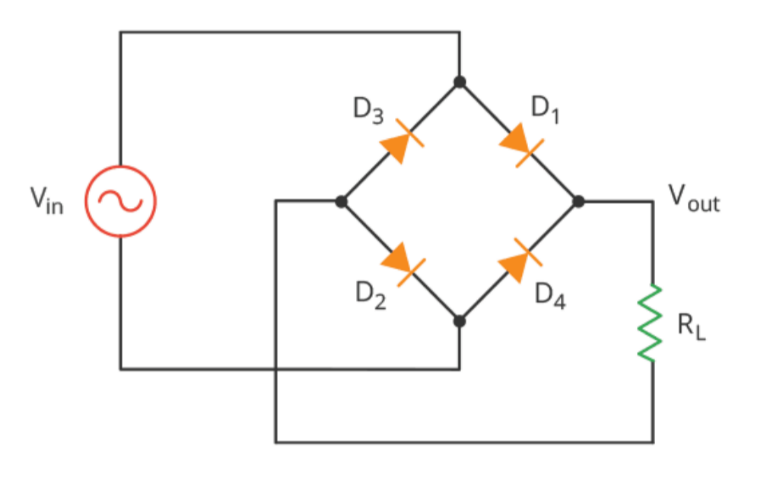
\includegraphics[width=0.6\textwidth]{Figures/Ch8/figure1.png}
    \setlength{\unitlength}{1mm}
    \caption{Full-Wave Bridge Rectifier}
    \label{fig:bridge_rectifier}
\end{figure}

\subsection{Netlist}
\begin{lstlisting}[caption=Full-Wave Bridge Rectifier Netlist]
* Full-Wave Bridge Rectifier  
Vin ac1 0 SIN(0 10 50)  
D1 ac1 out Dmod  
D2 0 out Dmod  
D3 gnd2 ac1 Dmod  
D4 gnd2 0 Dmod  
Rload out gnd2 1k  
.model Dmod D(IS=1e-14)  
.tran 100u 40m  
.end   
\end{lstlisting}

\subsection{Simulation Setup}
\begin{table}[H]
\centering
\caption{Full-Wave Bridge Rectifier Simulation Setup}
\begin{tabular}{ll}
\toprule
\textbf{Parameter} & \textbf{Value} \\
\midrule
Input Voltage & SIN(0 10 50) \\
Frequency & 50 Hz \\
Load Resistance & 1 k$\Omega$ \\
Analysis Type & Transient \\
\bottomrule
\end{tabular}
\end{table}

\subsection{Waveform Comparison}
Figure~\ref{fig:rectifier_dev_wave} shows the execution flow for the inductor, highlighting the parameter resolution, temperature scaling, and analysis-dependent matrix stamping. 

\begin{figure}[H]
    \centering
    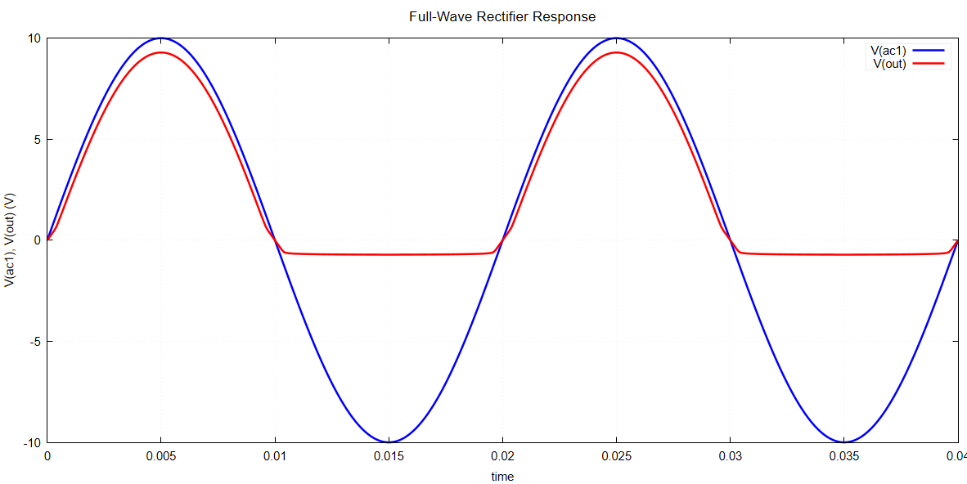
\includegraphics[width=0.6\textwidth]{Figures/Ch8/figure2.png}
    \caption{Output waveform generated by the developed simulator}
    \label{fig:rectifier_dev_wave}
\end{figure}


\begin{figure}[H]
    \centering
    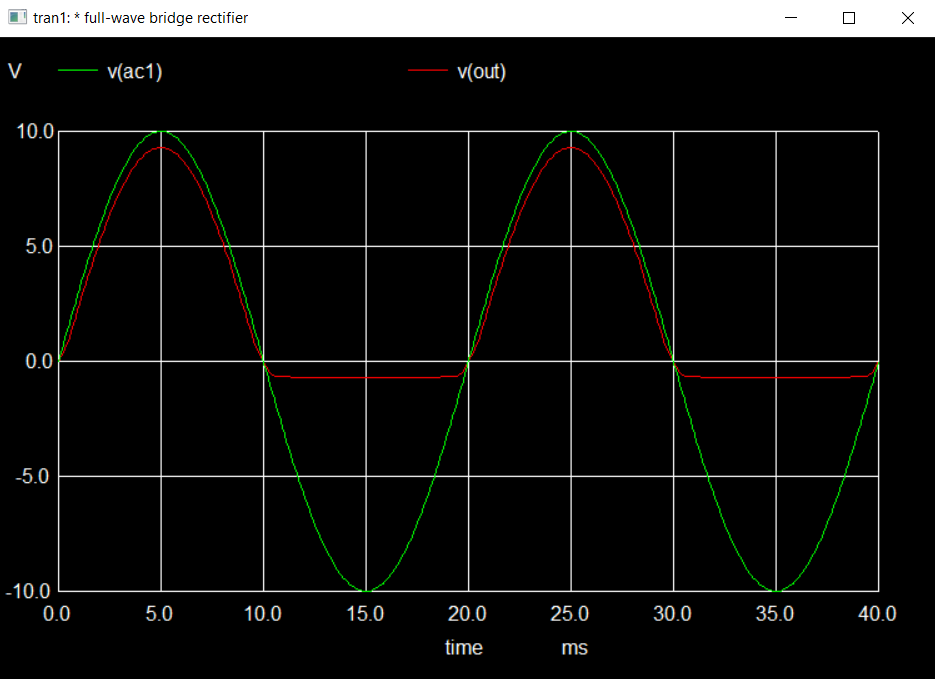
\includegraphics[width=0.6\textwidth]{Figures/Ch8/figure3.png}
    \caption{Output waveform generated by ngspice}
    \label{fig:rectifier_ngspice_wave}
\end{figure}

\subsection{Measurement Comparison}
\begin{table}[H]
\centering
\caption{Full-Wave Bridge Rectifier Measurement Comparison}
\small
\begin{tabular}{llll}
\toprule
\textbf{Measurement} & \textbf{\shortstack[l]{ngspice\\(Reference)}} & \textbf{\shortstack[l]{Developed simulator\\(Measured)}} & \textbf{\shortstack[l]{Relative\\error (\%)}} \\
\midrule
Maximum Voltage ($V_{\max}$) & 9.28891 V & 9.289291 V & 0.004 \\
Minimum Voltage ($V_{\min}$) & -0.710707 V & -0.7107088 V & 0.000253 \\
Peak-to-Peak Voltage ($V_{pp}$) & 9.999613 V & 10 V & 0.00387 \\
Average Voltage ($V_{\text{avg}}$) & 2.52046 V & 2.514236 V & 0.247 \\
RMS Voltage ($V_{\text{rms}}$) & 4.58304 V & 4.577338 V & 0.124 \\
Period & 20 msec & 20 msec & 0 \\
Frequency & 50 Hz & 50 Hz & 0 \\
\bottomrule
\end{tabular}
\end{table}


Relative error is computed as: 
\begin{equation}
\text{Error (\%)} = \frac{|\text{Reference} - \text{Measured}|}{|\text{Reference}|} \times 100
\end{equation}

\subsection{Conclusion}
The developed simulator successfully reproduced the expected behavior of the full-wave bridge rectifier. Comparison against ngspice showed strong agreement across all measured quantities. The maximum observed relative error was 0.247\% for the average output voltage, while all remaining measurements exhibited errors below 0.13\%. Overall, the results validate the correctness of the transient analysis engine, diode model implementation, and measurement subsystem for this benchmark circuit.


% ==========================================
% SECTION 2: COMMON-EMITTER AMPLIFIER
% ==========================================
\newpage
\section{Common-emitter Amplifier}

\subsection{Objective}
The purpose of this test is to validate the correctness of the BJT device model, DC operating point analysis, transient analysis engine, and post-processing measurement utilities using a common-emitter BJT amplifier. The results produced by the developed simulator are compared with those from ngspice.

\subsection{Circuit Description}
The test circuit is a single-stage common-emitter BJT NPN amplifier consisting of:
\begin{itemize}
    \item 12 V DC power supply
    \item Sinusoidal AC input voltage source
    \item Voltage-divider bias network ($R_1$ and $R_2$)
    \item NPN bipolar junction transistor (BJT)
    \item Collector resistor
    \item Emitter resistor with bypass capacitor
    \item Input and Output coupling capacitor
    \item Resistive load
\end{itemize}

\begin{figure}[H]
    \centering
    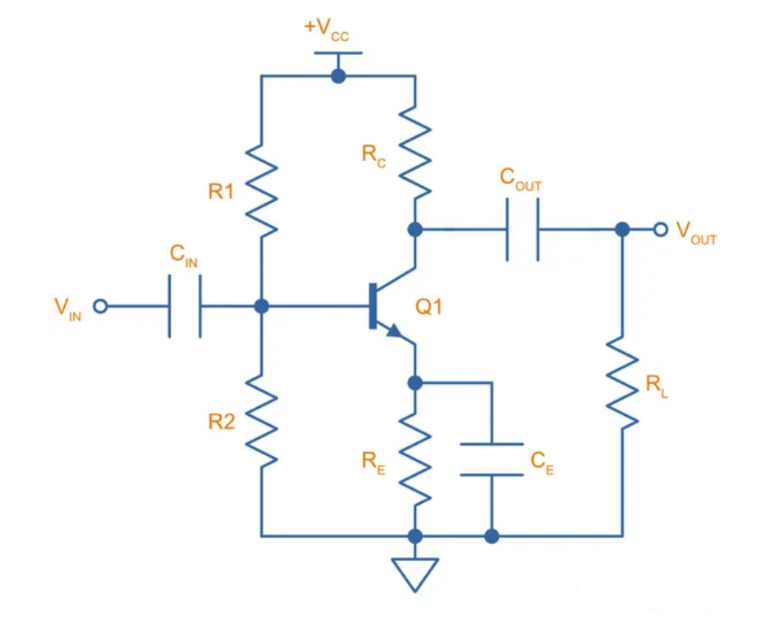
\includegraphics[width=0.6\textwidth]{Figures/Ch8/figure4.png}
    \caption{Common-emitter Amplifier}
    \label{fig:ce_amplifier}
\end{figure}

\subsection{Netlist}
\begin{lstlisting}[caption=BJT Common-Emitter Amplifier Netlist]
* BJT Common-Emitter Amplifier - Transient Test  
VCC VCC 0 DC 12  
* Input signal  
VIN IN 0 SIN(0 10m 1k)  
* Bias network  
R1 VCC B 100k  
R2 B 0 22k  
* Input coupling capacitor  
CIN IN B 10u  
* Collector resistor  
RC VCC C 2.2k  
* Emitter resistor  
RE E 0 1k  
* Emitter bypass capacitor  
CE E 0 100u  
* Output coupling capacitor  
COUT C OUT 10u  
* Load  
RL OUT 0 10k  
* Transistor  
Q1 C B E QMOD  
.model QMOD NPN (  
+ IS=1e-15  
+ BF=100  
+ VAF=100)  
.op  
.tran 1u 5m  
.end   
\end{lstlisting}

\subsection{Simulation Setup}
\begin{table}[H]
\centering
\caption{Common-Emitter Amplifier Simulation Setup}
\begin{tabular}{ll}
\toprule
\textbf{Parameter} & \textbf{Value} \\
\midrule
Supply Voltage & 12 V DC \\
Input Voltage & SIN(0 10m 1k) \\
Bias Network & $R_1 = 100\text{ k}\Omega$, $R_2 = 22\text{ k}\Omega$ \\
Collector Resistor ($RC$) & 2.2 k$\Omega$ \\
Emitter Resistor ($RE$) & 1 k$\Omega$ \\
Emitter Bypass Capacitor ($CE$) & 100 $\mu$F \\
Input Coupling Capacitor ($CIN$) & 10 $\mu$F \\
Output Coupling Capacitor ($COUT$) & 10 $\mu$F \\
Load Resistance ($RL$) & 10 k$\Omega$ \\
Transistor Model & NPN (BF = 100, IS = $1 \times 10^{-15}$ A, VAF = 100 V) \\
Analysis Type & DC Operating Point (.op) and Transient (.tran) \\
\bottomrule
\end{tabular}
\end{table}

\subsection{Waveform Comparison}
\begin{figure}[H]
    \centering
    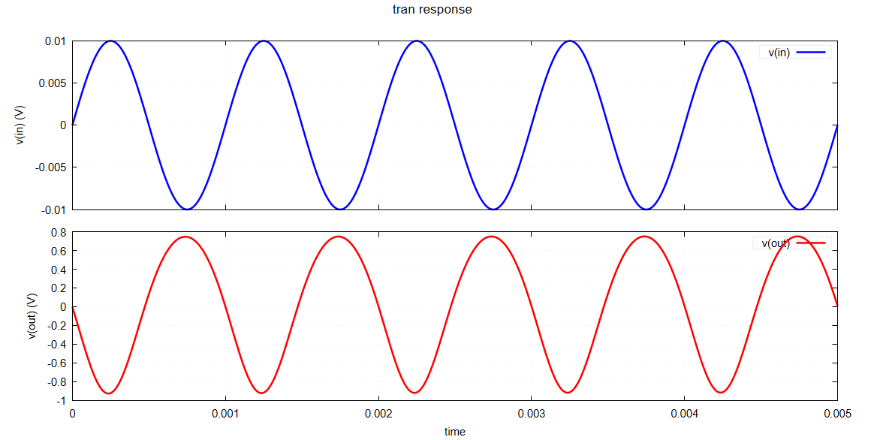
\includegraphics[width=0.6\textwidth]{Figures/Ch8/figure5.png}
    \caption{Output waveform generated by the developed simulator}
    \label{fig:ce_dev_wave}
\end{figure}

\begin{figure}[H]
    \centering
    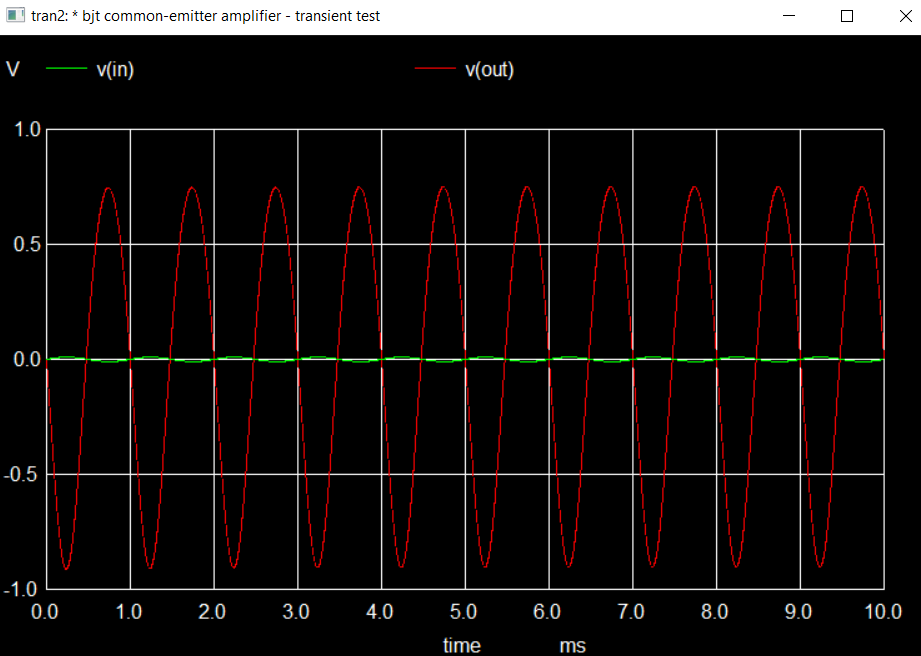
\includegraphics[width=0.6\textwidth]{Figures/Ch8/figure6.png}
    \caption{Output waveform generated by ngspice}
    \label{fig:ce_ngspice_wave}
\end{figure}

\subsection{Measurement Comparison}
\begin{table}[H]
\centering
\caption{Common-Emitter Amplifier Measurement Comparison}
\small
\begin{tabular}{llll}
\toprule
\textbf{Measurement} & \textbf{ngspice (Reference)} & \textbf{Developed simulator (Measured)} & \textbf{Relative error (\%)} \\
\midrule
$V_B$ (V) & 1.9576 V & 1.945137596 V & 0.637 \\
$V_C$ (V) & 9.2984 V & 9.330677592 V & 0.347 \\
$V_E$ (V) & 1.2395 V & 1.225461634 V & 1.13 \\
Maximum $V_{\text{in}}$ (V) & 9.99998 mV & 0.01 V & 0.0002 \\
Minimum $V_{\text{in}}$ (V) & -9.99998 mV & -0.01 V & 0.0002 \\
Peak-to-Peak $V_{\text{in}}$ (V) & 20 mV & 20 mV & 0 \\
Maximum $V_C$ (V) & 10.0474 V & 10.08238 V & 0.348 \\
Minimum $V_C$ (V) & 8.38502 V & 8.404955 V & 0.238 \\
Peak-to-Peak $V_C$ (V) & 1.66243 V & 1.677428 V & 0.902 \\
Average $V_C$ (V) & 9.29534 V & 9.325691 V & 0.327 \\
RMS $V_C$ (V) & 9.31367 V & 9.344306 V & 0.328 \\
Maximum $V_E$ (V) & 1.24101 V & 1.227032 V & 1.126 \\
Minimum $V_E$ (V) & 1.23946 V & 1.225462 V & 1.13 \\
Peak-to-Peak $V_E$ (V) & 1.544704 mV & 1.570768 mV & 1.7 \\
\bottomrule
\end{tabular}
\end{table}

\subsection{Conclusion}
The DC operating point and transient analysis results produced by the developed simulator show good agreement with the ngspice reference. The computed DC bias voltages closely match the reference operating point, confirming the correctness of the nonlinear device modeling and Newton–Raphson solution process. In transient analysis, the simulator accurately reproduces the amplifier's time-domain response, including waveform extrema, peak-to-peak values, average values, and RMS values. The relative errors are generally below 1\%, with a maximum error of approximately 1.7\%, demonstrating that the implemented BJT model, matrix stamping, DC operating point solver, and transient analysis algorithms operate correctly. Overall, the developed simulator accurately reproduces both the steady-state and dynamic behavior of the common-emitter BJT amplifier.



% ==========================================
% SECTION 3: COMMON-SOURCE MOSFET AMPLIFIER
% ==========================================
\newpage
\section{Common-Source MOSFET Amplifier}

\subsection{Objective}
The purpose of this test is to validate the correctness of the DC operating point solver, AC small-signal analysis engine, MOSFET device model implementation, and frequency response computation. The results produced by the developed simulator are compared with those from ngspice.
\subsection{Circuit Description}
The test circuit is a single-stage common-source NMOS amplifier consisting of:
\begin{itemize}
    \item 12 V DC power supply
    \item Sinusoidal AC input voltage source
    \item Voltage-divider gate bias network ($R_1$ and $R_2$)
    \item NMOS transistor
    \item Drain resistor
    \item Source resistor
    \item Input and output coupling capacitors
    \item Resistive load
\end{itemize}
\begin{figure}[H]
    \centering
    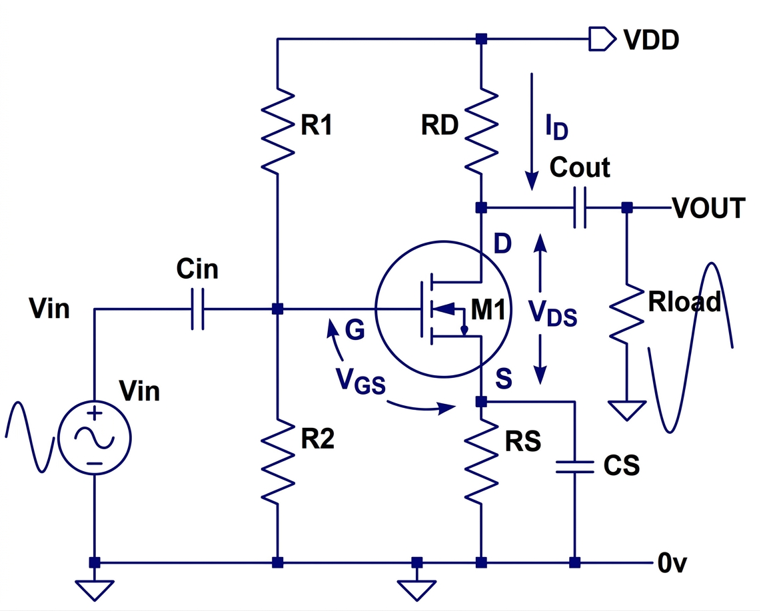
\includegraphics[width=0.6\textwidth]{Figures/Ch8/figure7.png}
    \caption{Common-source MOSFET Amplifier}
    \label{fig:cs_amplifier}
\end{figure}

\subsection{Netlist}
\begin{lstlisting}[caption=Standard NMOS Common-Source Amplifier Netlist]
    * Standard NMOS Common-Source Amplifier

    * Power Supply
    VDD VDD 0 DC 12V

    * Bias Network
    R1 VDD G 1Meg
    R2 G 0 470k

    * Drain and Source Resistors
    RD VDD D 4.7k
    RS S 0 1k

    * MOSFET
    * Drain Gate Source Bulk
    M1 D G S S nmos1 L=1u W=20u

    * Input and Output Coupling
    Cin in G 10u
    Cout D out 10u
    Rload out 0 10k

    * Input Signal
    * 10 mV Peak, 1 kHz
    Vin in 0 AC 1 SIN(0 10m 1k)

    * MOSFET Model
    .model nmos1 NMOS (LEVEL=1 VTO=1.5 KP=100u LAMBDA=0.02)

    .op
    .ac dec 10 10 100Meg
    .end

    .end
\end{lstlisting}

\subsection{Simulation Setup}
\begin{table}[H]
    \centering
    \caption{Common-Source MOSFET Amplifier Simulation Setup}
    \label{tab:cs_mosfet_setup}
    \begin{tabular}{lp{4.2in}}
        \toprule
        \textbf{Parameter} & \textbf{Value} \\
        \midrule
        Supply Voltage & 12 V DC \\
        Input Voltage & AC 1V, SIN(0 10m 1k) \\
        Bias Network & $R_1 = 1\text{ M}\Omega$, $R_2 = 470\text{ k}\Omega$ \\
        Drain Resistor ($RD$) & 4.7 k$\Omega$ \\
        Source Resistor ($RS$) & 1 k$\Omega$ \\
        Channel Dimensions & $\text{W} = 20\text{ \textmu m}$, $\text{L} = 1\text{ \textmu m}$ \\
        Input Coupling Capacitor ($CIN$) & 10 \textmu F \\
        Output Coupling Capacitor ($COUT$) & 10 \textmu F \\
        Load Resistance ($RL$) & 10 k$\Omega$ \\
        Transistor Model & NMOS Level 1 (VTO = 1.5 V, KP = 100 \textmu A/V$^2$, LAMBDA = 0.02) \\
        Analysis Type & DC Operating Point (.op) and AC (.ac) \\
        \bottomrule
    \end{tabular}
\end{table}



\subsection{Waveform Comparison}
\begin{figure}[H]
    \centering
    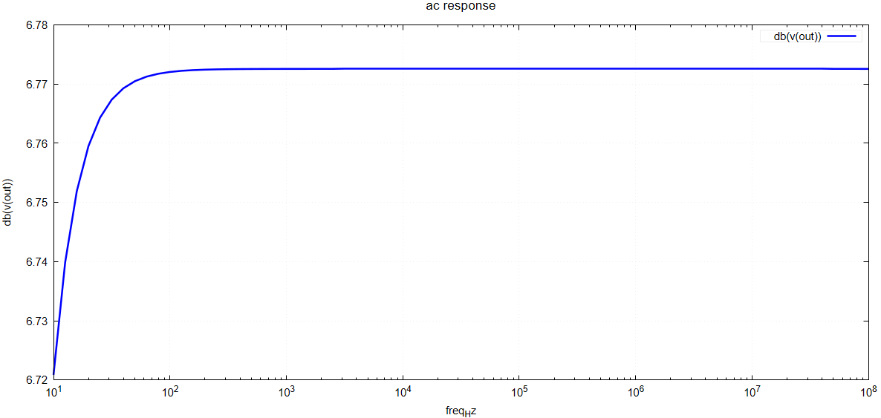
\includegraphics[width=0.6\textwidth]{Figures/Ch8/figure8.png}
    \caption{Gain (dB) waveform generated by the developed tool}
    \label{fig:ce_dev_wave}
\end{figure}

\begin{figure}[H]
    \centering
    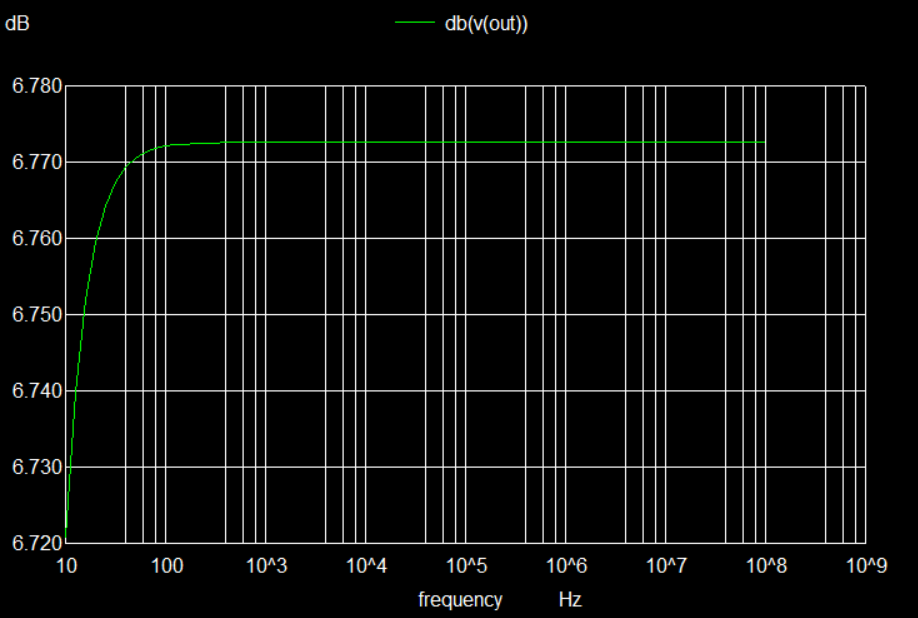
\includegraphics[width=0.6\textwidth]{Figures/Ch8/figure9.png}
    \caption{Gain (dB) waveform generated by ngspice}
    \label{fig:ce_dev_wave}
\end{figure}

\begin{figure}[H]
    \centering
    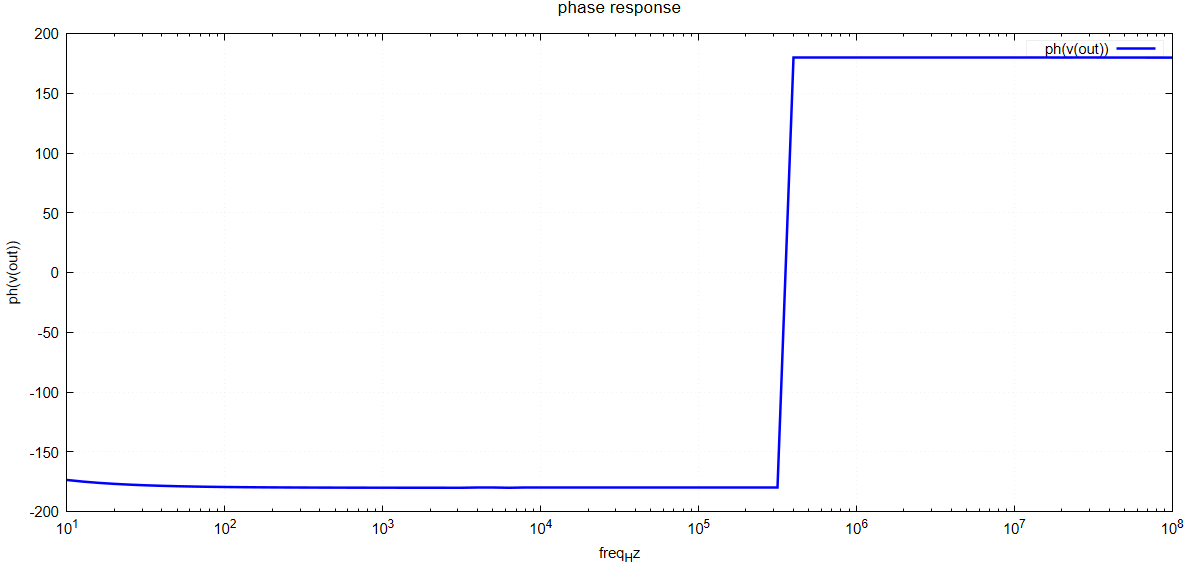
\includegraphics[width=0.6\textwidth]{Figures/Ch8/figure10.png}
    \caption{Phase (deg) waveform generated by the developed tool}
    \label{fig:ce_dev_wave}
\end{figure}

\begin{figure}[H]
    \centering
    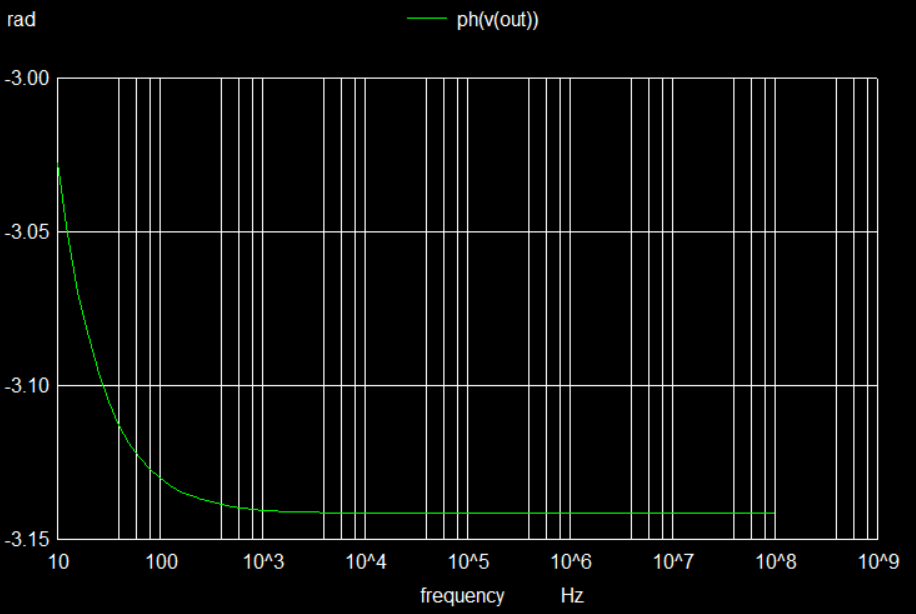
\includegraphics[width=0.6\textwidth]{Figures/Ch8/figure11.png}
    \caption{Phase (rad) waveform generated by ngspice}
    \label{fig:ce_dev_wave}
\end{figure}

\subsection{Measurement Comparison}
\begin{table}[H]
\centering
\caption{Common-Source MOSFET Amplifier Measurement Comparison}
\small
\begin{tabular}{llll}
\toprule
\textbf{Measurement} & \textbf{\shortstack[l]{ngspice\\(Reference)}} & \textbf{\shortstack[l]{Developed simulator\\(Measured)}} & \textbf{\shortstack[l]{Relative\\error (\%)}} \\
\midrule
$V_G$ (V) & 3.836735 V & 3.836733467 V & 0.00004 \\
$V_D$ (V) & 6.063083 V & 6.063087218 V & 0.00007 \\
$V_S$ (V) & 1.263174 V & 1.263172925 V & 0.00008 \\
$I_D$ (A) & 1.263174 mA & 1.271336 mA & 0.646 \\
Voltage Gain @ 1 kHz (dB) & 6.77257 dB & 6.772575 dB & 0 \\
Maximum Gain (dB) & 6.77258 dB & 6.772579 dB & 0.00001 \\
Maximum Output Magnitude (V) & 2.18087 V & 2.153867 V & 1.2 \\
\bottomrule
\end{tabular}
\end{table}



\subsection{Conclusion}
The developed simulator produced DC operating point and AC analysis results that closely matched the ngspice reference. The computed node voltages, drain current, and AC gain showed excellent agreement, with only minor numerical differences. These results validate the correctness of the implemented MOSFET Level-1 device model, DC operating point solver, and AC small-signal analysis engine.


% ==========================================
% SECTION 4: VCVS AMPLIFIER
% ==========================================
\newpage
\section{Voltage-Controlled Voltage Resistive Amplifier}

\subsection{Objective}
The purpose of this test is to validate the implementation of the Voltage-Controlled Voltage Source (VCVS) model, the controlled-source matrix stamping, and the DC operating point solver. The computed node voltages and source current are compared with the corresponding ngspice reference results to verify the correctness of the VCVS implementation.

\subsection{Circuit Description}
The test circuit consists of:
\begin{itemize}
    \item Independent DC voltage source
    \item Voltage-Controlled Voltage Source (VCVS)
    \item Input resistor
    \item Output voltage divider ($R_2$ and $R_3$)
\end{itemize}

\begin{figure}[H]
    \centering
    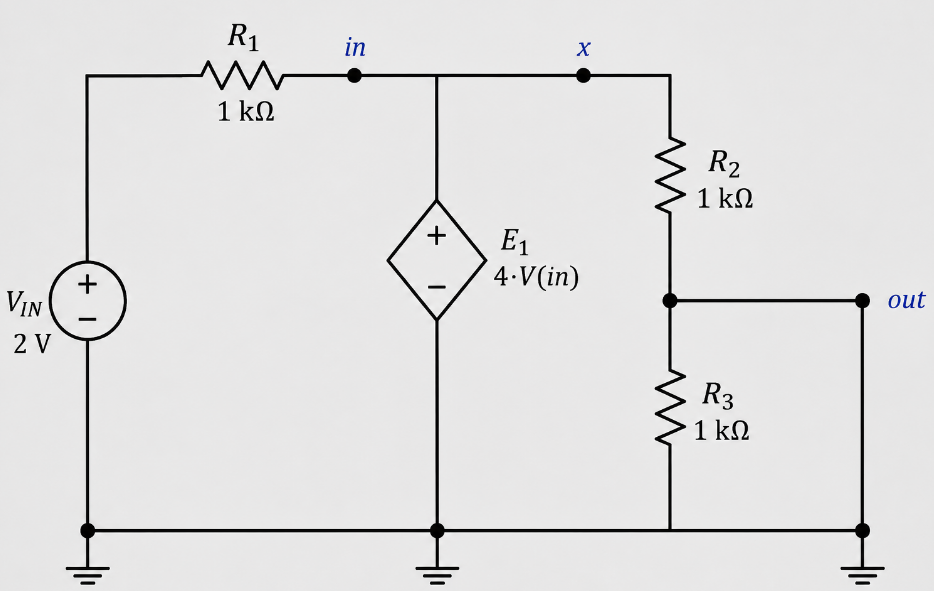
\includegraphics[width=0.6\textwidth]{Figures/Ch8/figure12.png}
    \caption{Voltage-Controlled Voltage Amplifier}
    \label{fig:vcvs_amplifier}
\end{figure}


\subsection{Netlist}
\begin{lstlisting}[caption=VCVS Amplifier Test Netlist]
* VCVS Amplifier Test  
VIN in 0 DC 2  
R1 in 0 1k  
E1 x 0 in 0 4  
R2 x out 1k  
R3 out 0 1k  
.op  
.end   
\end{lstlisting}

\subsection{Simulation Setup}
\begin{table}[H]
\centering
\caption{VCVS Resistive Amplifier Simulation Setup}
\label{tab:vcvs_setup}
\begin{tabular}{ll}
\toprule
\textbf{Parameter} & \textbf{Value} \\
\midrule
Supply Voltage    & 12 V DC \\
VCVS Gain         & 4 V/V \\
Input Resistance  & 1 k$\Omega$ \\
Output Resistance & 1 k$\Omega$ \\
Load Resistor     & 1 k$\Omega$ \\
Analysis Type     & DC Operating Point (.op) \\
\bottomrule
\end{tabular}
\end{table}

\subsection{Measurement Comparison}
\begin{table}[H]
\centering
\caption{VCVS Resistive Amplifier Measurement Comparison}
\label{tab:vcvs_comparison}
\begin{tabular}{llll}
\toprule
\textbf{Measurement} & \textbf{ngspice (Reference)} & \textbf{Developed simulator (Measured)} & \textbf{Relative error (\%)} \\
\midrule
$V_{\text{in}}$ (V)  & 2 V   & 2 V           & 0 \\
$V_x$ (V)            & 8 V   & 8 V           & 0 \\
$V_{\text{out}}$ (V) & 4 V   & 3.999999998 V & $\sim$0 \\
$I_{\text{vin}}$ (A) & -2 mA & -2 mA         & 0 \\
\bottomrule
\end{tabular}
\end{table}

Relative error is computed as: 
\begin{equation}
\text{Error (\%)} = \frac{|\text{Reference} - \text{Measured}|}{|\text{Reference}|} \times 100
\end{equation}

\subsection{Conclusion}
The developed simulator successfully reproduced the DC operating point of the VCVS resistive amplifier with virtually identical results to ngspice. Accurate computation of the controlled-source output voltage, node voltages, and source current confirms the correctness of the implemented VCVS model, controlled-source stamping, and DC operating-point solver.

% ==========================================
% SECTION 5: VCCS AMPLIFIER
% ==========================================
\newpage
\section{Voltage-Controlled Current Resistive Amplifier}

\subsection{Objective}
The purpose of this test is to validate the implementation of the Voltage-Controlled Current Source (VCCS) model, the controlled-source matrix stamping, and the DC operating point solver. The computed node voltages and source current are compared with the corresponding ngspice reference results to verify the correctness of the VCCS implementation.

\subsection{Circuit Description}
The test circuit consists of:
\begin{itemize}
    \item Independent DC voltage source
    \item Voltage-Controlled Current Source (VCCS)
    \item Input resistor
    \item Resistive load
\end{itemize}

\begin{figure}[H]
    \centering
    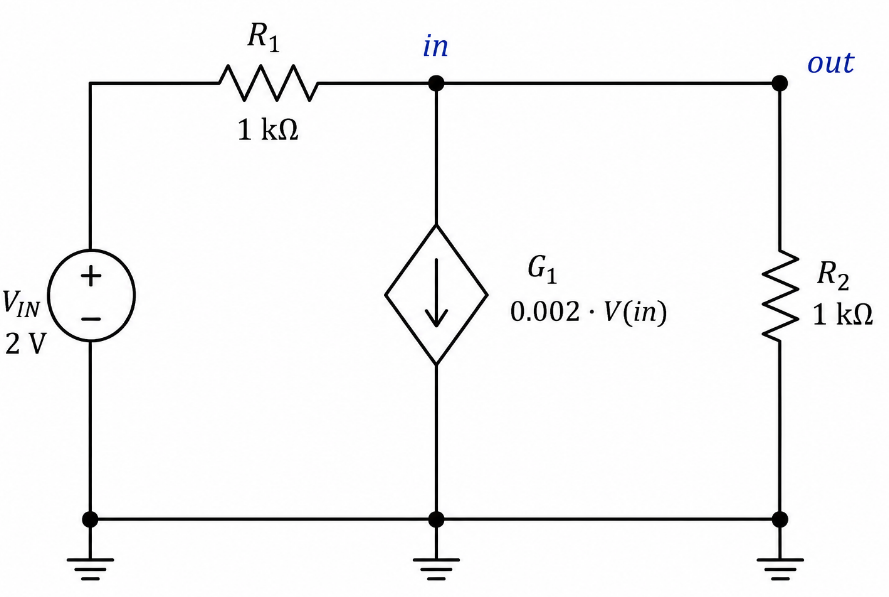
\includegraphics[width=0.6\textwidth]{Figures/Ch8/figure13.png}
    \caption{Voltage-Controlled Current Amplifier}
    \label{fig:vccs_amplifier}
\end{figure}


\subsection{Netlist}
\begin{lstlisting}[caption=VCCS Resistive Amplifier Netlist]
* VCCS Resistive Amplifier  
VIN in 0 DC 2  
* Input resistor  
R1 in 0 1k  
* VCCS: Gname N+ N- NC+ NC- Gain  
G1 out 0 in 0 0.002  
* Load resistor  
R2 out 0 1k  
.op  
.end   
\end{lstlisting}

\subsection{Simulation Setup}
\begin{table}[H]
\centering
\caption{VCCS Resistive Amplifier Simulation Setup}
\label{tab:vccs_setup}
\begin{tabular}{ll}
\toprule
\textbf{Parameter} & \textbf{Value} \\
\midrule
Supply Voltage        & 12 V DC \\
VCCS Transconductance & 2 mS \\
Input Resistance      & 1 k$\Omega$ \\
Load Resistor         & 1 k$\Omega$ \\
Analysis Type         & DC Operating Point (.op) \\
\bottomrule
\end{tabular}
\end{table}

\subsection{Measurement Comparison}
\begin{table}[H]
\centering
\caption{VCCS Resistive Amplifier Measurement Comparison}
\label{tab:vccs_comparison}
\begin{tabular}{llll}
\toprule
\textbf{Measurement} & \textbf{ngspice (Reference)} & \textbf{Developed simulator (Measured)} & \textbf{Relative error (\%)} \\
\midrule
$V_{\text{in}}$ (V)  & 2 V   & 2 V           & 0 \\
$V_{\text{out}}$ (V) & -4 V  & -3.999999998 V & $\sim$0 \\
$I_{\text{vin}}$ (A) & -2 mA & -2 mA         & 0 \\
\bottomrule
\end{tabular}
\end{table}

\subsection{Conclusion}
The developed simulator successfully reproduced the DC operating point of the VCCS resistive amplifier with virtually identical results to ngspice. Accurate computation of the controlled-source output voltage, node voltages, and source current confirms the correctness of the implemented VCCS model, controlled-source stamping, and DC operating-point solver.

% ==========================================
% SECTION 6: CCCS AMPLIFIER
% ==========================================
\newpage
\section{Current-Controlled Current Resistive Amplifier}

\subsection{Objective}
The purpose of this test is to validate the implementation of the Current-Controlled Current Source (CCCS) model, the controlled-source matrix stamping, and the DC operating point solver. The computed node voltages and source current are compared with the corresponding ngspice reference results to verify the correctness of the CCCS implementation.

\subsection{Circuit Description}
The test circuit consists of:
\begin{itemize}
    \item Independent DC voltage source
    \item Current-sensing voltage source
    \item Current-Controlled Current Source (CCCS)
    \item Input resistor
    \item Resistive load
\end{itemize}

\begin{figure}[H]
    \centering
    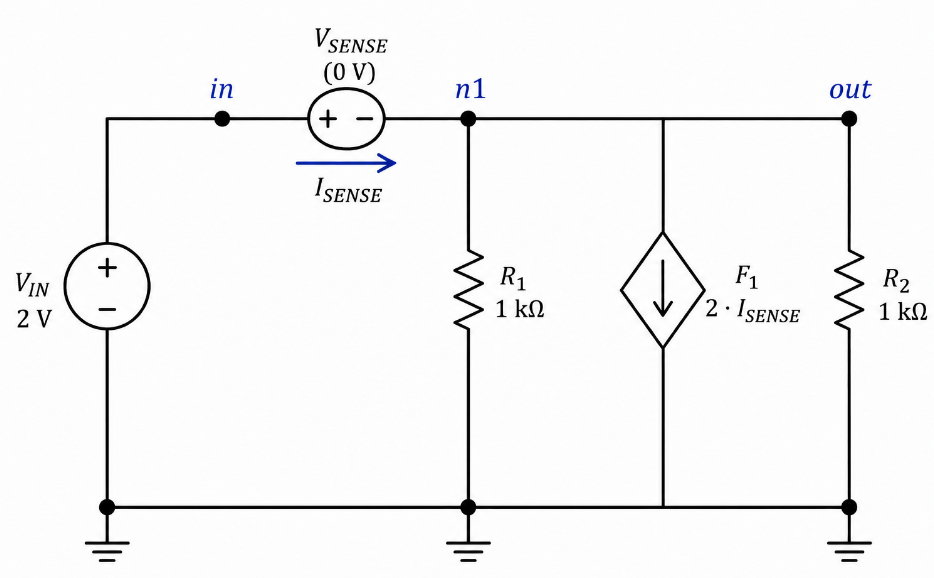
\includegraphics[width=0.6\textwidth]{Figures/Ch8/figure14.png}
    \caption{Current-controlled Current Amplifier}
    \label{fig:cccs_amplifier}
\end{figure}

\subsection{Netlist}
\begin{lstlisting}[caption=CCCS Resistive Amplifier Netlist]
* CCCS Resistive Amplifier  
VIN in 0 DC 2  
* Current sensing source  
VSENSE in n1 DC 0  
* Input resistor  
R1 n1 0 1k  
* CCCS: Fname N+ N- Vname Gain  
F1 out 0 VSENSE 2  
* Load resistor  
R2 out 0 1k  
.op  
.end   
\end{lstlisting}

\subsection{Simulation Setup}
\begin{table}[H]
\centering
\caption{CCCS Resistive Amplifier Simulation Setup}
\label{tab:cccs_setup}
\begin{tabular}{ll}
\toprule
\textbf{Parameter} & \textbf{Value} \\
\midrule
Supply Voltage   & 12 V DC \\
CCCS Gain        & 2 A/A \\
Input Resistance & 1 k$\Omega$ \\
Load Resistor    & 1 k$\Omega$ \\
Analysis Type    & DC Operating Point (.op) \\
\bottomrule
\end{tabular}
\end{table}

\subsection{Measurement Comparison}
\begin{table}[H]
\centering
\caption{CCCS Resistive Amplifier Measurement Comparison}
\label{tab:cccs_comparison}
\begin{tabular}{llll}
\toprule
\textbf{Measurement} & \textbf{\shortstack[l]{ngspice\\(Reference)}} & \textbf{\shortstack[l]{Developed simulator\\(Measured)}} & \textbf{\shortstack[l]{Relative\\error (\%)}} \\
\midrule
$V_{\text{in}}$ (V)  & 2 V   & 2 V     & 0 \\
$V_{\text{out}}$ (V) & -4 V  & -4 V    & 0 \\
$I_{\text{vin}}$ (A) & -2 mA & -2 mA   & 0 \\
\bottomrule
\end{tabular}
\end{table}

\subsection{Conclusion}
The developed simulator successfully reproduced the DC operating point of the CCCS resistive amplifier, yielding results identical to ngspice. Accurate computation of the controlled-source output current, node voltages, and source current confirms the correctness of the implemented CCCS model, controlled-source stamping, and DC operating-point solver.

% ==========================================
% SECTION 7: CCVS AMPLIFIER
% ==========================================
\newpage
\section{Current-Controlled Voltage Resistive Amplifier}

\subsection{Objective}
The purpose of this test is to validate the implementation of the Current-Controlled Voltage Source (CCVS) model, the controlled-source matrix stamping, and the DC operating point solver. The computed node voltages and source current are compared with the corresponding ngspice reference results to verify the correctness of the CCVS implementation.

\subsection{Circuit Description}
The test circuit consists of:
\begin{itemize}
    \item Independent DC voltage source
    \item Current-sensing voltage source
    \item Current-Controlled Voltage Source (CCVS)
    \item Input resistor
    \item Resistive load
\end{itemize}

\begin{figure}[H]
    \centering
    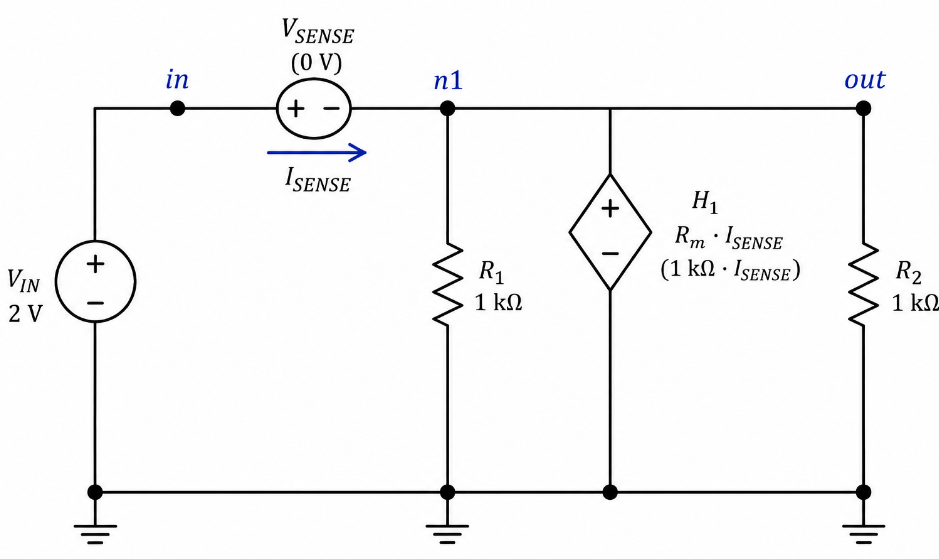
\includegraphics[width=0.6\textwidth]{Figures/Ch8/figure15.png}
    \caption{Current-controlled Voltage Amplifier}
    \label{fig:ccvs_amplifier}
\end{figure}


\subsection{Netlist}
\begin{lstlisting}[caption=CCVS Resistive Amplifier Netlist]
* CCVS Resistive Amplifier  
VIN in 0 DC 2  
* Current sensing source  
VSENSE in n1 DC 0  
* Input resistor  
R1 n1 0 1k  
* CCVS: Hname N+ N- Vname Gain (ohms)  
H1 out 0 VSENSE 1000  
* Load resistor  
R2 out 0 1k  
.op  
.end   
\end{lstlisting}

\subsection{Simulation Setup}
\begin{table}[H]
\centering
\caption{CCVS Resistive Amplifier Simulation Setup}
\label{tab:ccvs_setup}
\begin{tabular}{ll}
\toprule
\textbf{Parameter} & \textbf{Value} \\
\midrule
Supply Voltage        & 12 V DC \\
CCVS Transresistance & 1 k$\Omega$ \\
Input Resistance      & 1 k$\Omega$ \\
Load Resistor         & 1 k$\Omega$ \\
Analysis Type         & DC Operating Point (.op) \\
\bottomrule
\end{tabular}
\end{table}

\subsection{Measurement Comparison}
\begin{table}[H]
\centering
\caption{CCVS Resistive Amplifier Measurement Comparison}
\label{tab:ccvs_comparison}
\begin{tabular}{llll}
\toprule
\textbf{Measurement} & \textbf{ngspice (Reference)} & \textbf{Developed simulator (Measured)} & \textbf{Relative error (\%)} \\
\midrule
$V_{\text{in}}$ (V)  & 2 V   & 2 V     & 0 \\
$V_{\text{out}}$ (V) & 2 V   & 2 V     & 0 \\
$I_{\text{vin}}$ (A) & -2 mA & -2 mA   & 0 \\
\bottomrule
\end{tabular}
\end{table}

\subsection{Conclusion}
The developed simulator successfully reproduced the DC operating point of the CCVS resistive amplifier with identical results to ngspice. Accurate computation of the controlled-source output voltage, node voltages, and source current confirms the correctness of the implemented CCVS model, controlled-source stamping, and DC operating-point solver.

% ==========================================
% SECTION 8: SERIES RLC CIRCUIT
% ==========================================
\newpage
\section{Series RLC Circuit}

\subsection{Objective}
The purpose of this test is to validate the implementation of the inductor model, the resistor and capacitor device models, and the transient analysis engine. The computed transient response of the RLC circuit is compared with the corresponding ngspice reference results to verify the correctness of the implemented device models and numerical integration algorithm.

\subsection{Circuit Description}
The test circuit is a series RLC mesh topology consisting of:
\begin{itemize}
    \item Pulse voltage source
    \item Series resistor
    \item Series inductor
    \item Capacitor connected to ground
\end{itemize}

\begin{figure}[H]
    \centering
    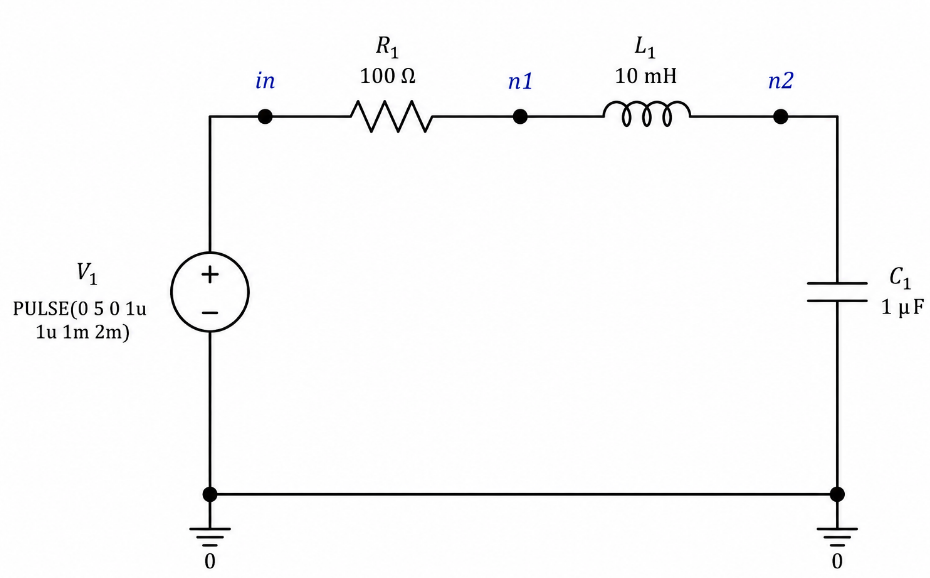
\includegraphics[width=0.6\textwidth]{Figures/Ch8/figure16.png}
    \caption{Series RLC Circuit}
    \label{fig:series_rlc}
\end{figure}


\subsection{Netlist}
\begin{lstlisting}[caption=Series RLC Transient Response Netlist]
* Series RLC Transient Response  
V1 in 0 PULSE(0 5 0 1u 1u 1m 2m)  
R1 in n1 100  
L1 n1 n2 10m  
C1 n2 0 1u  
.tran 10u 10m  
.end   
\end{lstlisting}

\subsection{Simulation Setup}
\begin{table}[H]
\centering
\caption{Series RLC Circuit Simulation Setup}
\label{tab:rlc_setup}
\begin{tabular}{ll}
\toprule
\textbf{Parameter} & \textbf{Value} \\
\midrule
Input Voltage & PULSE(0 V, 5 V, 0, 1 $\mu$s, 1 $\mu$s, 1 ms, 2 ms) \\
Resistance    & 100 $\Omega$ \\
Inductance    & 10 mH \\
Capacitance   & 1 $\mu$F \\
Analysis Type & Transient (.tran) \\
\bottomrule
\end{tabular}
\end{table}

\subsection{Waveform Comparison}
\begin{figure}[H]
    \centering
    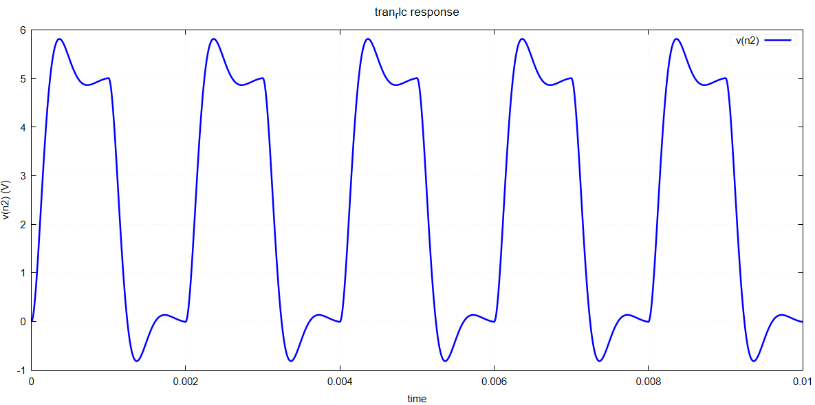
\includegraphics[width=0.6\textwidth]{Figures/Ch8/figure17.png}
    \caption{Output waveform generated by the developed simulator}
    \label{fig:rlc_dev_wave}
\end{figure}

\begin{figure}[H]
    \centering
    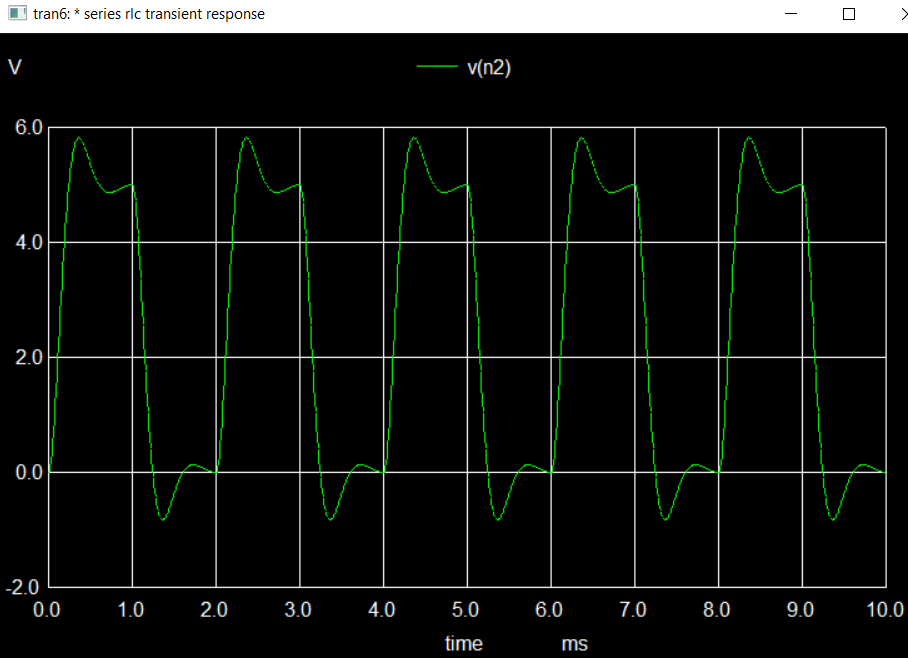
\includegraphics[width=0.6\textwidth]{Figures/Ch8/figure18.png}
    \caption{Output waveform generated by ngspice}
    \label{fig:rlc_ngspice_wave}
\end{figure}


\subsection{Measurement Comparison}
\begin{table}[H]
\centering
\caption{Series RLC Circuit Measurement Comparison}
\label{tab:rlc_comparison}
\small
\begin{tabular}{llll}
\toprule
\textbf{Measurement} & \textbf{\shortstack[l]{ngspice\\(Reference)}} & \textbf{\shortstack[l]{Developed simulator\\(Measured)}} & \textbf{\shortstack[l]{Relative\\error (\%)}} \\
\midrule
Maximum Capacitor Voltage (V) & 5.81848 V   & 5.817099 V   & 0.024 \\
Minimum Capacitor Voltage (V) & -8.18603 V  & -8.170151 V  & 0.194 \\
Peak-to-Peak Voltage (V)       & 6.63708 V   & 6.634114 V   & 0.0447 \\
Final Capacitor Voltage (V)   & -10.4023 mV & -10.17337 mV & 2.2 \\
Average Capacitor Voltage (V) & 2.50288 V   & 2.501084 V   & 0.072 \\
RMS Capacitor Voltage (V)     & 3.53595 V   & 3.534223 V   & 0.0488 \\
\bottomrule
\end{tabular}
\end{table}


\subsection{Conclusion}
The developed simulator successfully reproduced the transient response of the series RLC circuit with results closely matching the ngspice reference. These results validate the correctness of the implemented resistor, capacitor, and inductor models, as well as the transient analysis engine and numerical integration algorithm.

% ==========================================
% SECTION 9: COMMON-GATE JFET AMPLIFIER
% ==========================================
\newpage
\section{Common-gate JFET Amplifier}

\subsection{Objective}
The purpose of this test is to validate the implementation of the Junction Field-Effect Transistor (JFET) model, the nonlinear device stamping, the DC operating point solver, and the AC small-signal analysis engine. The computed operating-point voltages, drain current, and AC gain are compared with the corresponding ngspice reference results to verify the correctness of the implemented JFET model.

\subsection{Circuit Description}
The test circuit is a single-stage common-gate JFET amplifier consisting of:
\begin{itemize}
    \item 12 V DC power supply
    \item N-channel JFET
    \item Gate bias network
    \item Drain resistor
    \item Source resistor
    \item Input coupling capacitor
    \item Output coupling capacitor
    \item Resistive load
    \item Sinusoidal AC input source
\end{itemize}

\begin{figure}[H]
    \centering
    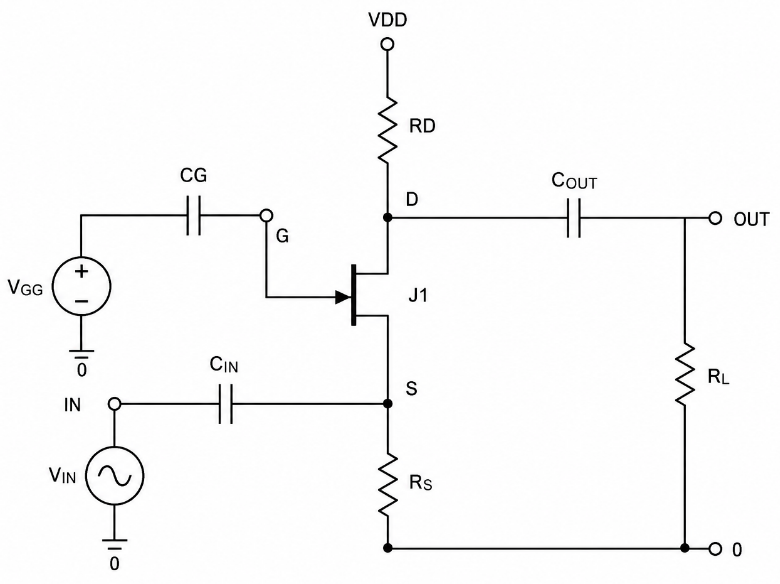
\includegraphics[width=0.6\textwidth]{Figures/Ch8/figure19.png}
    \caption{Common-gate JFET Amplifier}
    \label{fig:jfet_amplifier}
\end{figure}

\newpage
\subsection{Netlist}
\begin{lstlisting}[caption=JFET Common-Gate Amplifier Netlist]
* JFET Common-Gate Amplifier  
* Power Supply  
VDD VDD 0 DC 12  
* Gate Bias (AC Ground)  
VGG G 0 DC 2  
CG G 0 100u  
* Input Signal  
VIN IN 0 AC 1 SIN(0 10m 1k)  
* Input Coupling  
CIN IN S 10u  
* Drain and Source Resistors  
RD VDD D 4.7k  
RS S 0 470  
* Output Coupling  
COUT D OUT 10u  
RL OUT 0 10k  
* JFET  
* Drain Gate Source  
J1 D G S JMOD  
* JFET Model  
.model JMOD NJF (  
+ VTO=-2  
+ BETA=1m  
+ LAMBDA=0.02)  
* Analyses  
.op  
.ac dec 10 10 100Meg  
.end   
\end{lstlisting}

\subsection{Simulation Setup}
\begin{table}[H]
\centering
\caption{Common-Gate JFET Amplifier Simulation Setup}
\label{tab:jfet_setup}
\begin{tabular}{lp{4.2in}}
\toprule
\textbf{Parameter} & \textbf{Value} \\
\midrule
Supply Voltage                     & 12 V DC \\
Input Voltage                      & AC 1V, SIN(0 10m 1k) \\
Gate Bias                          & 2 V DC \\
Drain Resistor ($R_{\text{D}}$)    & 4.7 k$\Omega$ \\
Source Resistor ($R_{\text{S}}$)   & 470 $\Omega$ \\
Gate Bypass Capacitor ($C_{\text{G}}$) & 100 \textmu F \\
Input Coupling Capacitor ($C_{\text{IN}}$) & 10 \textmu F \\
Output Coupling Capacitor ($C_{\text{OUT}}$) & 10 \textmu F \\
Load Resistance ($R_{\text{L}}$)   & 10 k$\Omega$ \\
Transistor Model                   & N-Channel JFET (VTO = -2 V, BETA = 1 mA/V$^2$, LAMBDA = 0.02) \\
Analysis Type                      & DC Operating Point (.op) and AC (.ac) \\
\bottomrule
\end{tabular}
\end{table}


\subsection{Waveform Comparison}
\begin{figure}[H]
    \centering
    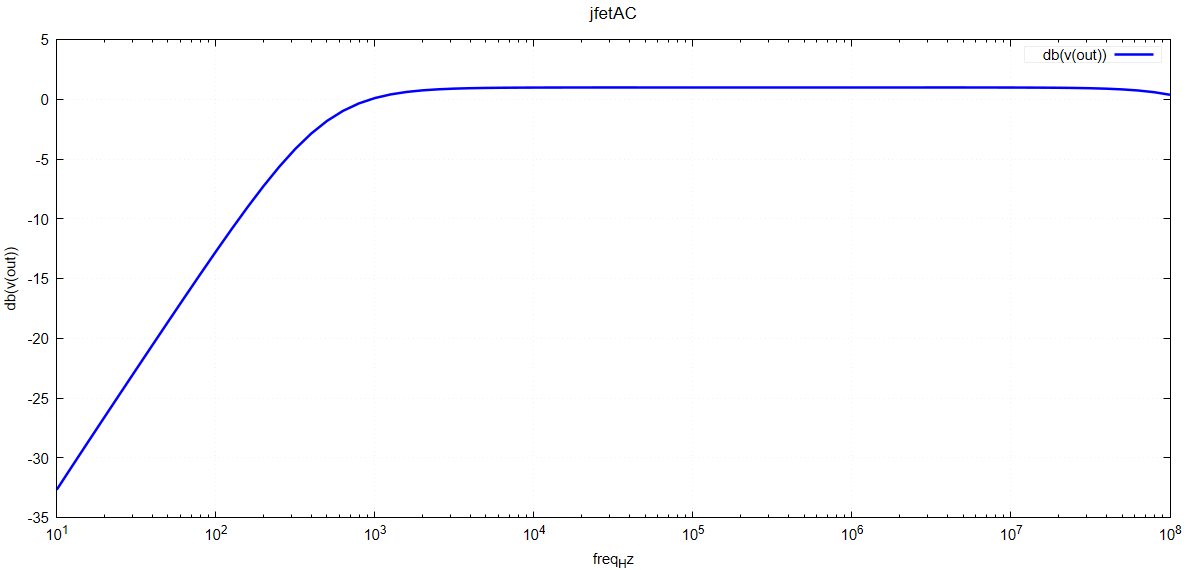
\includegraphics[width=0.6\textwidth]{Figures/Ch8/figure20.png}
    \caption{Gain (dB) waveform generated by the developed simulator}
    \label{fig:jfet_dev_gain}
\end{figure}

\begin{figure}[H]
    \centering
    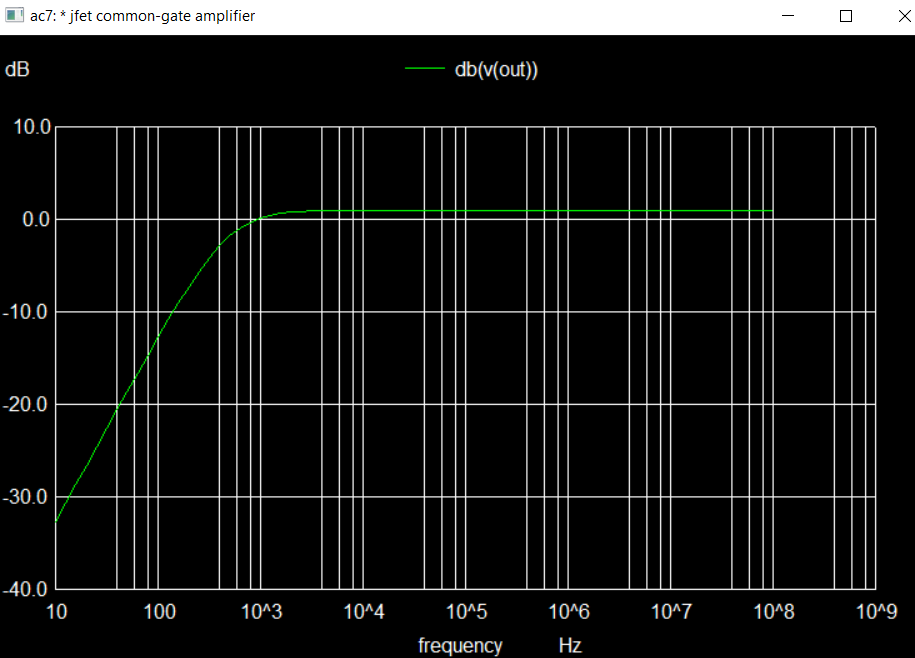
\includegraphics[width=0.6\textwidth]{Figures/Ch8/figure22.png}
    \caption{Gain (dB) waveform generated by ngspice}
    \label{fig:jfet_ngspice_gain}
\end{figure}

\begin{figure}[H]
    \centering
    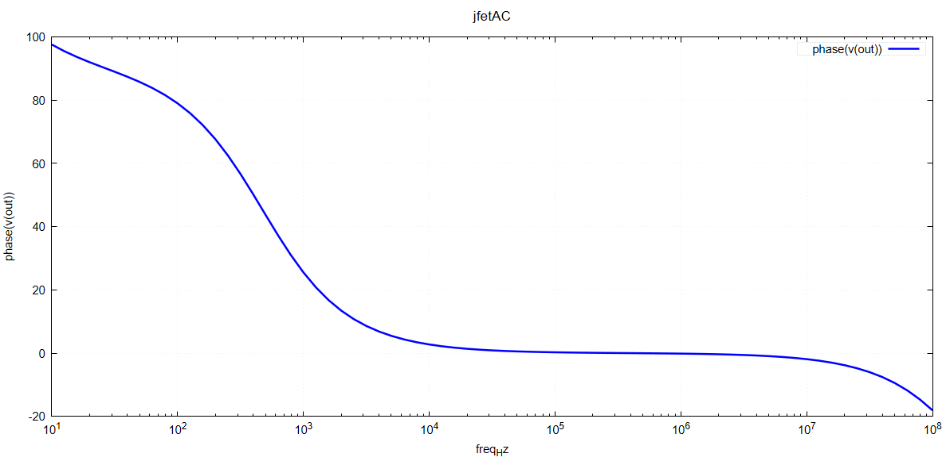
\includegraphics[width=0.6\textwidth]{Figures/Ch8/figure21.png}
    \caption{Phase (deg) waveform generated by the developed simulator}
    \label{fig:jfet_dev_phase}
\end{figure}

\begin{figure}[H]
    \centering
    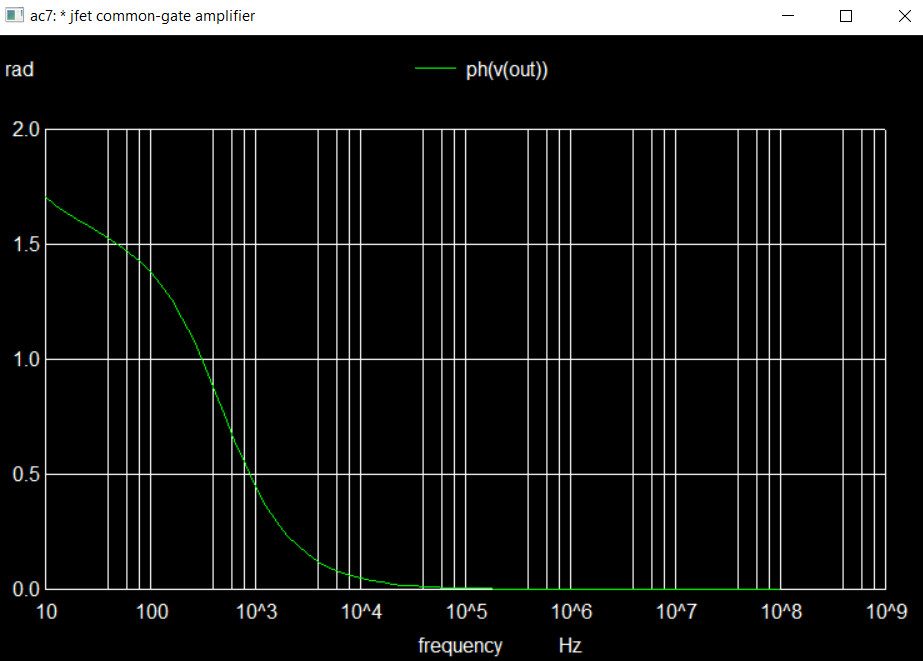
\includegraphics[width=0.6\textwidth]{Figures/Ch8/figure23.png}
    \caption{Phase (rad) waveform generated by ngspice}
    \label{fig:jfet_ngspice_phase}
\end{figure}

\subsection{Measurement Comparison}
\begin{table}[H]
\centering
\caption{Common-Gate JFET Amplifier Measurement Comparison}
\label{tab:jfet_comparison}
\resizebox{\textwidth}{!}{%
\begin{tabular}{llll}
\toprule
\textbf{Measurement} & \textbf{ngspice (Reference)} & \textbf{Developed simulator (Measured)} & \textbf{Relative error (\%)} \\
\midrule
$V_G$ (V)                     & 2 V          & 2 V            & 0 \\
$V_D$ (V)                     & 1.79751 V    & 1.797509236 V  & 0 \\
$V_S$ (V)                     & 1.353756 V   & 1.35375498 V   & 0.00008 \\
$I_D$ (A)                     & 2.170743 mA  & 2.170743 mA    & 0 \\
Voltage Gain @ 1 kHz (dB)     & 0.107839 dB  & 0.1112338 dB   & 3 \\
Maximum Gain (dB)             & 0.995071 dB  & 0.998477 dB    & 0.34 \\
Maximum Output Magnitude (V)  & 1.12138 V    & 1.121822 V     & 0.0394 \\
\bottomrule
\end{tabular}%
}
\end{table}

\subsection{Conclusion}
The developed simulator successfully reproduced the DC operating point and AC response of the JFET common-gate amplifier with results closely matching the ngspice reference. The computed node voltages and drain current were virtually identical to the reference values, while the AC gain and output magnitude exhibited only minor numerical differences. These results validate the correctness of the implemented JFET model, nonlinear device stamping, DC operating-point solver, and AC small-signal analysis engine.

% ===============================================
% SECTION 10: CMOS Low-Dropout Voltage Regulator 
% ===============================================

\newpage
\section{CMOS Low-Dropout (LDO) Voltage Regulator}

\subsection{Objective}
The purpose of this test is to validate the simulator's ability to handle a relatively large nonlinear CMOS circuit, including multiple MOSFET devices, passive components, and feedback networks. The operating-point solution is compared against ngspice to verify the correctness of the nonlinear device models, matrix assembly, and Newton-Raphson solver. This test also evaluates the simulator's scalability for larger circuits.

\subsection{Circuit Description}
The test circuit is a CMOS Low-Dropout (LDO) voltage regulator consisting of:
\begin{itemize}
    \item 3.3 V DC input supply
    \item 1.2 V reference voltage source
    \item PMOS differential error amplifier
    \item NMOS active load
    \item CMOS driver stage
    \item PMOS pass transistor
    \item Resistive feedback divider
    \item Output capacitor
    \item Resistive load
\end{itemize}

\begin{figure}[H]
    \centering
    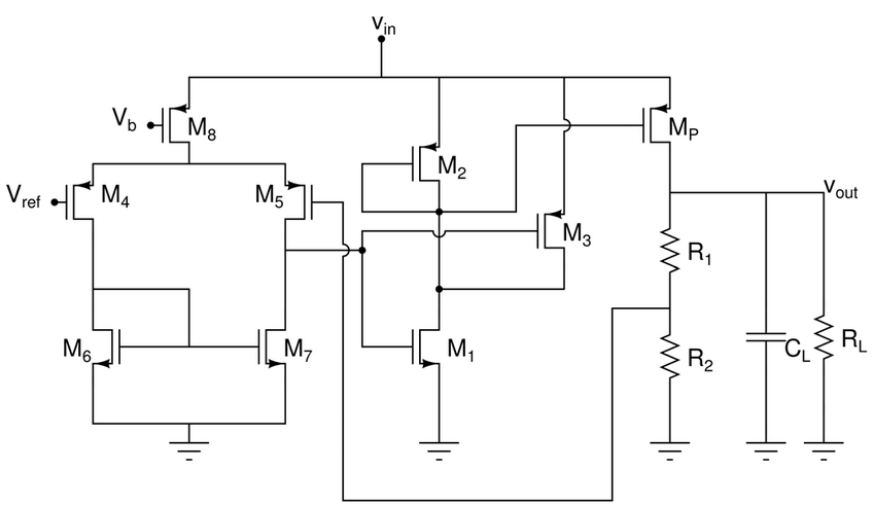
\includegraphics[width=0.6\textwidth]{Figures/Ch8/figure24.png}
    \caption{Common-gate JFET Amplifier}
    \label{fig:jfet_amplifier}
\end{figure}

\subsection{Netlist}
\begin{lstlisting}[caption={CMOS LDO Voltage Regulator Circuit Netlist}]
* CMOS LDO Voltage Regulator Circuit Netlist
* --- Power Supplies & Inputs ---
Vin vin 0 PULSE(0 3.3 0 1u 1u 20m 40m)
Vref vref 0 DC 1.2
Vb vb 0 DC 2.0

* --- Error Amplifier (Differential Stage & Active Load) ---
M8 tail n_ea_out vin vin PMOS W=10u L=0.5u
M4 n_load vref tail vin PMOS W=20u L=0.5u
M5 n_ea_out fb tail vin PMOS W=20u L=0.5u
M6 n_load n_load 0 0 NMOS W=10u L=0.5u
M7 n_ea_out n_load 0 0 NMOS W=10u L=0.5u

* --- Intermediate Buffer / Driver Stage ---
M1 n_gate_mp n_ea_out 0 0 NMOS W=15u L=0.5u
M2 n_gate_mp n_ea_out vin vin PMOS W=30u L=0.5u
M3 n_gate_mp n_ea_out vin vin PMOS W=30u L=0.5u

* --- Power Pass Element ---
Mp vout n_gate_mp vin vin PMOS W=500u L=0.5u

* --- Feedback Voltage Divider ---
R1 vout fb 100k
R2 fb 0 100k

* --- Output Load Components ---
CL vout 0 1u
RL vout 0 100

* --- Simulation Commands ---
.op

* --- Model Placeholders ---
.model NMOS nmos (level=1 VTO=0.7 KP=100U LAMBDA=0.02)
.model PMOS pmos (level=1 VTO=-0.7 KP=50U LAMBDA=0.02)
.end
\end{lstlisting}

\subsection{Simulation Setup}
\begin{table}[H]
    \centering
    \caption{CMOS LDO Voltage Regulator Simulation Setup}
    \label{tab:ldo_setup}
    \begin{tabular}{lp{4in}}
        \toprule
        \textbf{Parameter} & \textbf{Value} \\
        \midrule
        Supply Voltage & PULSE(0 V, 3.3 V, 0, 1 \textmu s, 1 \textmu s, 20 ms, 40 ms) \\
        Reference Voltage & 1.2 V DC \\
        Bias Voltage & 2.0 V DC \\
        Feedback Resistors & 100 k$\Omega$ / 100 k$\Omega$ \\
        Output Capacitor & 1 \textmu F \\
        Load Resistance & 100 $\Omega$ \\
        Pass Transistor & PMOS ($W = 500\text{ \textmu m}$, $L = 0.5\text{ \textmu m}$) \\
        PMOS MOSFET Model & NMOS Level 1 ($V_{\text{TO}} = 1.5\text{ V}$, $KP = 50\,\mu\text{A/V}^2$, $\lambda = 0.02$) \\
        NMOS MOSFET Model & NMOS Level 1 ($V_{\text{TO}} = 1.5\text{ V}$, $KP = 100\,\mu\text{A/V}^2$, $\lambda = 0.02$) \\
        Analysis Type & DC Operating Point (.op) \\
        \bottomrule
    \end{tabular}
\end{table}

\subsection{Measurement Comparison}
\begin{table}[H]
    \centering
    \caption{CMOS LDO Voltage Regulator Measurement Comparison}
    \label{tab:ldo_comparison}
    \small
    \begin{tabular}{llll}
        \toprule
        \textbf{Measurement} & \textbf{\shortstack[l]{ngspice\\(Reference)}} & \textbf{\shortstack[l]{Developed simulator\\(Measured)}} & \textbf{\shortstack[l]{Relative\\error (\%)}} \\
        \midrule
        $V_{\text{vin}}$ (V) & 3.3 V & 3.3 V & -- \\
        $V_{\text{vref}}$ (V) & 1.2 V & 1.2 V & -- \\
        $V_{\text{vb}}$ (V) & 2 V & 2 V & -- \\
        $V_{\text{tail}}$ (V) & 2.198524 V & 2.1985234 V & 0.00002 \\
        $V_{\text{n\_load}}$ (V) & 0.99911 V & 0.99911 V & 0 \\
        $V_{\text{n\_ea\_out}}$ (V) & 1.81318 V & 1.81318 V & 0 \\
        $V_{\text{n\_gate\_mb}}$ (V) & 1.62874 V & 1.62874 V & 0 \\
        $V_{\text{fb}}$ (V) & 1.19521 V & 1.19521 V & 0 \\
        $V_{\text{vout}}$ (V) & 2.39041 V & 2.39041 V & 0 \\
        \bottomrule
    \end{tabular}
\end{table}

\subsection{Conclusion}
The developed simulator successfully analyzed the CMOS LDO voltage regulator and accurately computed its DC operating point. The measured node voltages and regulated output matched the ngspice reference results, confirming the correctness of the implemented MOSFET models, nonlinear device stamping, matrix assembly, and Newton-Raphson DC solver. In addition to validating the operating-point solution, this circuit served as a large-scale benchmark, demonstrating the simulator's ability to handle a more complex design containing multiple MOSFETs, passive components, and a feedback network. The agreement with the reference simulator verifies both the accuracy and scalability of the developed simulation engine for larger nonlinear circuits.


% ==========================================
% SECTION 11: Performance Evaluation
% ==========================================
\newpage
\section{Performance Evaluation}
\begin{table}[H]
    \centering
    \caption{Performance Evaluation of Benchmark Circuits}
    \label{tab:performance_evaluation}
    \small
    % This wrapper guarantees the table matches your page margins exactly
    \resizebox{\textwidth}{!}{%
    \begin{tabular}{lcccc}
        \toprule
        \textbf{Benchmark Circuit} & \textbf{\shortstack[c]{Simulation\\runtime (msec)}} & \textbf{\shortstack[c]{Current Memory\\(MB)}} & \textbf{\shortstack[c]{Peak Memory\\(MB)}} & \textbf{\shortstack[c]{Private Memory\\(MB)}} \\
        \midrule
        Full-Wave Rectifier                 & 45  & 9.5  & 9.51  & 0.8  \\
        Common-emitter Amplifier            & 99  & 4.52 & 5.25  & 1.23 \\
        Common-source MOSFET Amplifier      & 2   & 4.33 & 4.34  & 0.75 \\
        Voltage-Controlled Voltage Amplifier & 5   & 4.05 & 4.06  & 0.67 \\
        Voltage-Controlled Current Amplifier & 5   & 4.07 & 4.080 & 0.71 \\
        Current-Controlled Current Amplifier & 2   & 4.06 & 4.07  & 0.71 \\
        Current-Controlled Voltage Amplifier & 6   & 4.06 & 4.07  & 0.7  \\
        Series RLC                          & 212 & 4.19 & 4.3   & 0.79 \\
        Common-gate JFET Amplifier          & 9   & 4.16 & 4.16  & 0.69 \\
        CMOS LDO Voltage Regulator          & 9  & 4.53   & 4.54    & 0.85   \\
        \bottomrule
    \end{tabular}%
    }
\end{table}

